\documentclass[a4paper,11pt]{article}

\usepackage[T1]{fontenc}
\usepackage[utf8]{inputenc}
\usepackage[english,polish]{babel}
\usepackage{lmodern}
\usepackage{graphicx}
\usepackage{fancyhdr}
\usepackage{float}
\usepackage{array}

%\usepackage{mathtools}


\setlength{\textheight}{23.5cm}
\setlength{\textwidth}{15.92cm}
\setlength{\footskip}{10mm}
\setlength{\oddsidemargin}{0mm}
\setlength{\evensidemargin}{0mm}
\setlength{\topmargin}{0mm}
\setlength{\headsep}{15mm}
\setlength{\parindent}{0cm}
\setlength{\parskip}{2.5mm}
\author{Justyna Ilczuk, Jacek Rosiński}

\begin{document}

\begin{center}

    \begin{tabular}{ | m{5cm}| m{5cm} | m{5cm} |}
    \hline 
    \multicolumn{2}{|c|}{Elektronika w eksperymencie fizycznym}
    & Rok akademicki 2012-2013 \\ 
    
    \hline
    Środa 14.15-17.00 
    & Justyna Ilczuk \newline Jacek Rosiński
    & Wykonane w dniu 17.04.2013 \\
   	
   	\hline
   	Ćwiczenie 8 & Elementy i układy przełączające &    Ocena: \\
   	\hline
    \end{tabular}
\end{center}

%\newpage
\pagestyle{fancy}
\fancyfoot[CO]{\ }
\fancyhead[RO]{\footnotesize{\thepage} }
%\fancyhead[RO]{\footnotesize{\ } }
\fancyhead[LO]{Justyna Ilczuk i Jacek Rosiński K-1, Elementy i układy przełączające }




\section{Cel ćwiczenia}
Celem ćwiczenia było poznanie parametrów przełączników elektryczych oraz zasad działania elektroniczych układów przełączających.

\section{Użyty sprzęt i układy pomiarowe}

Hardware:
\begin{itemize}
\item komputer PC
\item Elvis II+
\item Oporniki o odpowiednich wartościach,
\item Multimetr METEX M3610,
\item Tranzystor,
\item Diody: prostownicza 1N4007 i przełączająca 1N4148
\item Przełącznik elektromechaniczny
\item Kondensatory: C i \(C_L\), 

\end{itemize}

Software:
\begin{itemize}
\item oprogramowanie od National Instruments do pomiarów na Elvisie

\end{itemize}

\section{Wstęp teoretyczny}

Idalnym przełącznikiem można określić takie urządzenie, podczas włączenia posiada zerową oporność, zaś podczas wyłączenia jego oporność w nieskończenie małym czasie zmienia się na nieskończoną. W układach rzeczywistych taka sytuacja nie ma miejsca. Przełączniki podczas włączenia posiadają oporność, zaś podczas wyłącznia przepływa przez nie niewielki prąd. Ponadto przełącznik posiada swoją pojemność. Stąd bierze się sporo efektów niepożądanych, które to badamy w tym doświadczeniu. W naszym doświadczeniu jako przełącznikiem posługiwaliśmy się układami: 
\begin{figure} [H]
  \begin{center}
    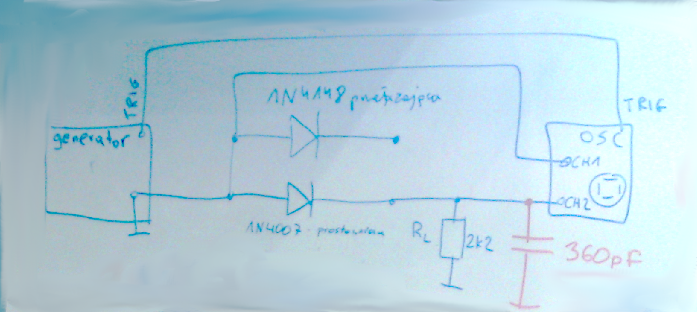
\includegraphics[width = 10cm]{../Obrazki_i_tekst/obrobione/u1.png}
    \caption{Układ 1}
  \end{center}
\end{figure}
Gdzie badaliśmy dwie diody podpisane na schemacie. Dzięki otrzymanym tak przebiegom można wyznaczyć czas wyłączania 
 $ t_{OFF} = t_1 + t_2 $ (rysunek 3) diody, a także oszacować największą częstotliwość, przy której dioda przestaje pracować jako przełącznik.  Układ pobudzamy sygnałem prostokątnym o częstotliwości $50 kHz$ i napięciu $V_{pp}=	5 V$.



\begin{figure} [H]
  \begin{center}
    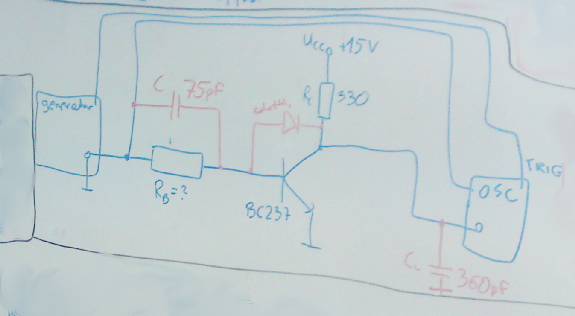
\includegraphics[width = 10cm]{../Obrazki_i_tekst/obrobione/u2.png}
    \caption{Układ 2}
  \end{center}
\end{figure}
Układu drugiego użyliśmy, aby badać wpływ elementów oznaczonych na kolor czerwony w naszyk układzie pobudzanym sygnałem prostokątnym. Opór $R_B$ został wyznaczony następująco: 

\( V_{pp}=	3,5 V, \ f=50 kHz, \)
\( U_c= 15 V, \ \beta  =100, \) 
\( I_c= \frac {U_{cc}} {R_c}, \)
\( U_{BE} = 0,7 V \) \newline
\(  I_c=\beta \cdot I_B, \ U_{CE}=0,1 V \)
\( R_B= \frac {E_g -U_{BE}} {I_B}  \)
$$ R_B = \frac {3,5-0,7}{15} \cdot 330 \cdot 100 = 6160 \Omega $$
Wybraliśmy opornik najbliższy pożądanej wartości, czyli $6k2$.

\begin{figure} [H]
  \begin{center}
    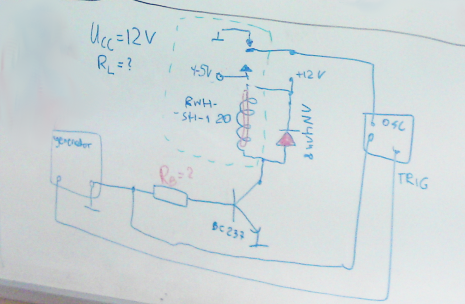
\includegraphics[width = 10cm]{../Obrazki_i_tekst/obrobione/u3.png}
    \caption{Układ 3}
  \end{center}
\end{figure}
Układ trzeci, przełącznik elektromechaniczny, pobudzamy początokowo częstotliwością $3 Hz$ i napięciem $V_{pp}=	3,5 V$. Dodatkowo do układu doprowadzamy napięcie $U_{cc} = 12 V $. Z pomiaru omomierzem otrzymujemy opór cewki $ R_L = 406 \Omega$, który posłuży do obliczenia oporu $R_B$. Poza tym drobnym szczegółem obliczneia wyglądają analogicznie.
$$ R_B = \frac {3,5-0,7}{12} \cdot 406 \cdot 100 = 9473,3 \Omega $$
Wybraliśmy opornik najbliższy pożądanej wartości, czyli $9k2$.

Ważnym momentem w analizie odpowiedzi układu jest zbadanie czasów zmiany sygnału czyli na przykład 
\begin{figure} [H]
  \begin{center}
    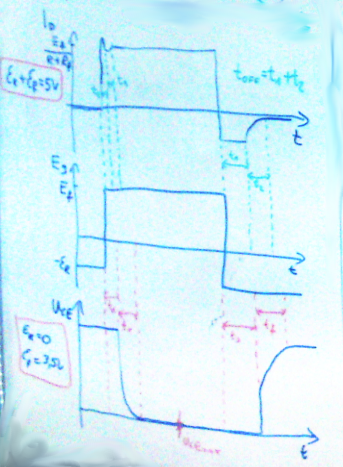
\includegraphics[width = 7cm]{../Obrazki_i_tekst/obrobione/w1.png}
    \caption{Przykładowe sygnały i zaznaczone w nich sektory interesujące}
  \end{center}
\end{figure}





\section{Opracowanie wyników}


\subsection{Badanie diod jako przełączników}
Na początku (w części pierwszej) badaliśmy układy przełączające z diodami, poniżej przedstawiamy zmierzone przebiegi dla częstotliwości 50 kHz.

Na poniższych rysunkach 1 kratka pozioma oznacza \(2 \mu s\).

W podpisach rysunków używamy \(E_F \) i \(E_R \) oraz \(U_{max} \)

\(U_{max} = E_F - E_R = 5V_{p-p}\)


Żeby się nie powtarzać: przy pomiarze czasów występuje niepewność, wynikająca z odczytu pomiaru, którą szacujemy na 1/10 podziałki, co w praktyce oznacza w przełożeniu na używane przez nas jednostki, że niepewność ta dla każdego odczytu czasu wynosi \(0.2 \mu s\).

Dla diody prostowniczej:

\begin{figure} [H]
  \begin{center}
    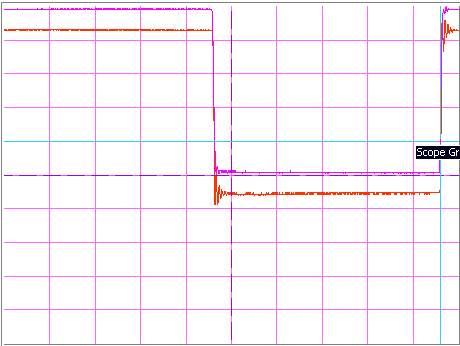
\includegraphics[width = 9cm]{../Obrazki_i_tekst/obrobione/1asciety.png}
    \caption{\( E_F = U_{max}, \ E_R = 0V \)}
  \end{center}
\end{figure}

Dla tego przypadku \( t_{off} \) praktycznie można pominąć, bo nie sposób wyznaczyć go na podstawie przebiegu.

\begin{figure} [H]
  \begin{center}
    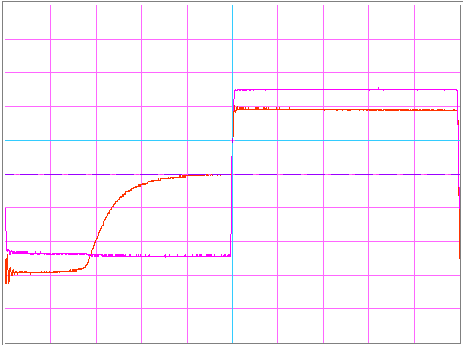
\includegraphics[width = 9cm]{../Obrazki_i_tekst/obrobione/1bsciety.png}
    \caption{\( E_F = 0.5 U_{max}, \ E_R = -0.5 U_{max}\)}
  \end{center}
\end{figure}

Gdy zmieniliśmy offset napięcia tak, że przełącznik był wyłączany napięciem - 2.5 V, sytuacja zdecydowanie się zmieniła i zaobserwowaliśmy następujące czasy wyłączania diody:

 \(t_1 = 3.6 \mu s,\ t_2 = 4.4 \mu s,\ t_{off} = 8 \mu s \).

\begin{figure} [H]
  \begin{center}
    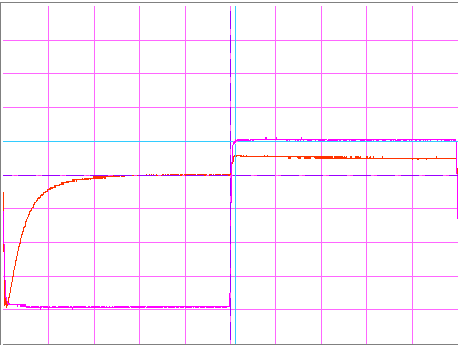
\includegraphics[width = 9cm]{../Obrazki_i_tekst/obrobione/1csciety.png}
    \caption{\( E_F = 1V, \ E_R = -4 V\)}
  \end{center}
\end{figure}

Dalej zmieniając offset, zauważamy, że charakterystyka przebiegu się zmienia i że t1, traci kosztem t2:

 \(t_1 = 0 \mu s,\ t_2 = 5 \mu s,\ t_{off} = 5 \mu s \).

\begin{figure} [H]
  \begin{center}
    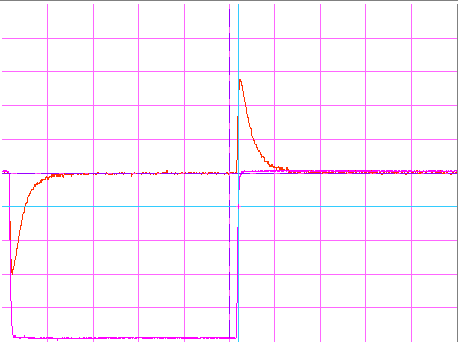
\includegraphics[width = 9cm]{../Obrazki_i_tekst/obrobione/1dsciety.png}
    \caption{\( E_F = 1V, \ E_R = -4 V\)}
  \end{center}
\end{figure}

Dalej zmieniając offset, tak że napięcie sterujące jest mniejsze, równe 0V, obserwujemy, że dioda nie zachowuje się uż jako przełącznik.

\begin{figure} [H]
  \begin{center}
    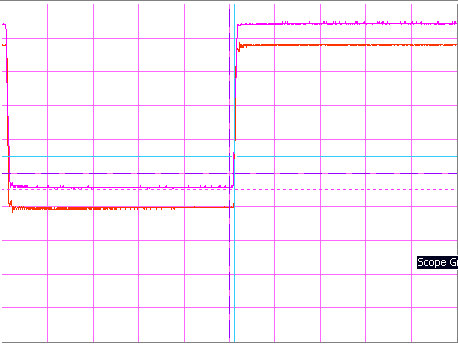
\includegraphics[width = 9cm]{../Obrazki_i_tekst/obrobione/1esciety.png}
    \caption{\( E_F = U_{max}, \ E_R = 0V \) z dołączonym kondensatorem \(C_L = 360 pF\)}
  \end{center}
\end{figure}

Ten układ różni się od pierwszego jedynie dołączonym kondensatorem \(C_L = 360 pF\). Nie dziwi zatem, że jego odpowiedź jest bardzo podobna do pierwszego układu, jeśli chodzi o różnice to, można zauważyć, że oscylacje na diodzie są mniejsze, ale poza tym jest praktycznie identycznie i czas wyłączania diody jest podobnie mały, tak że nie ma sensu go mierzyć.

Wszystkie poprzednie pomiary były przeprowadzone dla częstotliwości 50 kHz. Naszym kolejnym zadaniem było oszacowanie najmniejszej częstotliwości, przy której dioda przestaje pracować jako przełącznik.

\begin{figure} [H]
  \begin{center}
    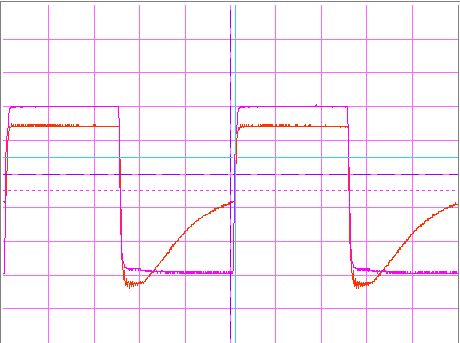
\includegraphics[width = 9cm]{../Obrazki_i_tekst/obrobione/2ciety.png}
    \caption{\( E_F = U_{max}, \ E_R = 0V \) dla częstotliwości 99 kHz }
  \end{center}
\end{figure}


Powyższy przebieg wyraźnie wskazuje, że dioda nie pracuje tu już jako przełącznik ponieważ cały czas płynie przez nią prąd w dwie strony i nie ma chwili, kiedy prąd przez nią nie płynie, czyli ani przez chwilę nie jest naprawdę wyłączona.

\textbf{Analogiczne badania przeprowadziliśmy dla diody impulsowej.}




\begin{figure} [H]
  \begin{center}
    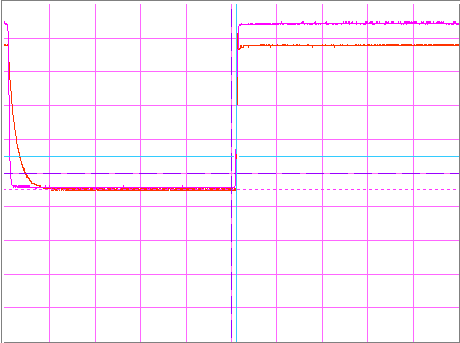
\includegraphics[width = 9cm]{../Obrazki_i_tekst/obrobione/31asciety.png}
    \caption{\( E_F = U_{max}, \ E_R = 0V \)}
  \end{center}
\end{figure}

Dla tego przypadku \( t_{off} \) jest stosunkowo niewielki.

\(t_1 = 0 \mu s,\ t_2 = 1.2 \mu s,\ t_{off} = 1.2 \mu s \).

\begin{figure} [H]
  \begin{center}
    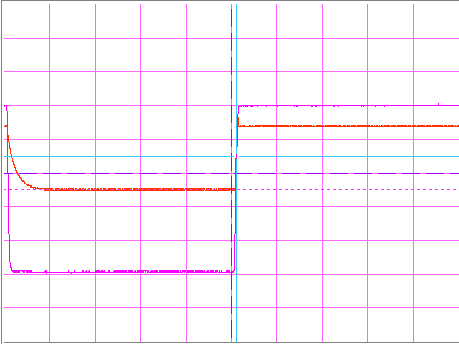
\includegraphics[width = 9cm]{../Obrazki_i_tekst/obrobione/31bsciety.png}
    \caption{\( E_F = 0.5 U_{max}, \ E_R = -0.5 U_{max}\)}
  \end{center}
\end{figure}

Gdy zmieniliśmy offset napięcia tak, że przełącznik był wyłączany napięciem - 2.5 V, czas wyłaczania diody praktycznie nie uległ zmianie:

\(t_1 = 0 \mu s,\ t_2 = 1.2 \mu s,\ t_{off} = 1.2 \mu s \).

\begin{figure} [H]
  \begin{center}
    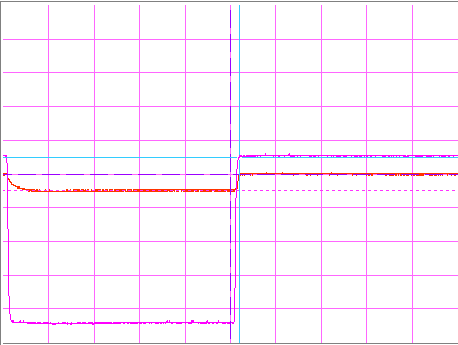
\includegraphics[width = 9cm]{../Obrazki_i_tekst/obrobione/31csciety.png}
    \caption{\( E_F = 1V, \ E_R = -4 V\)}
  \end{center}
\end{figure}

Dalej zmieniając offset, zauważamy, że zakres napięcia w którym przełącza dioda jest coraz mniejszy, czasy oszacowaliśmy następująco:

 \(t_1 = 0 \mu s,\ t_2 = 0.8 \mu s,\ t_{off} = 0.8 \mu s \).

\begin{figure} [H]
  \begin{center}
    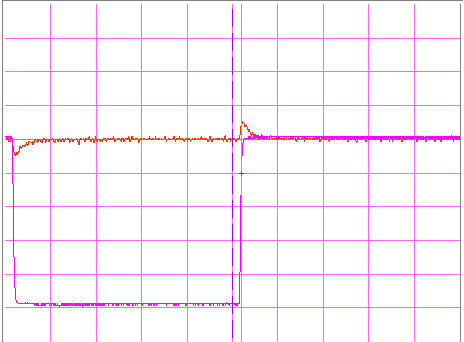
\includegraphics[width = 9cm]{../Obrazki_i_tekst/obrobione/31dsciety.png}
    \caption{\( E_F = 1V, \ E_R = -4 V\)}
  \end{center}
\end{figure}

Dalej zmieniając offset, tak że napięcie sterujące jest mniejsze, równe 0V, obserwujemy, że dioda nie zachowuje się uż jako przełącznik.

\begin{figure} [H]
  \begin{center}
    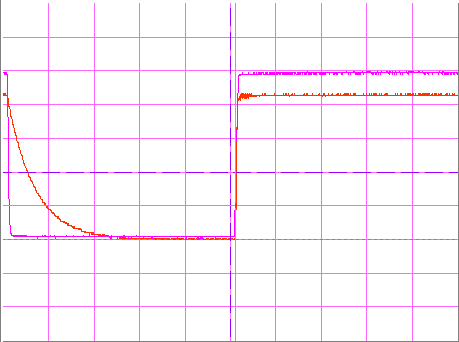
\includegraphics[width = 9cm]{../Obrazki_i_tekst/obrobione/31esciety.png}
    \caption{\( E_F = U_{max}, \ E_R = 0V \) z dołączonym kondensatorem \(C_L = 360 pF\)}
  \end{center}
\end{figure}

Ten układ różni się od pierwszego z diodą impulsową jedynie dołączonym kondensatorem \(C_L = 360 pF\). Jego odpowiedź jest bardzo podobna do pierwszego układu, ale czas \( t_2 \) zauważalnie się zwiększył.

\(t_1 = 0 \mu s,\ t_2 = 4 \mu s,\ t_{off} = 4 \mu s \).

\begin{figure} [H]
  \begin{center}
    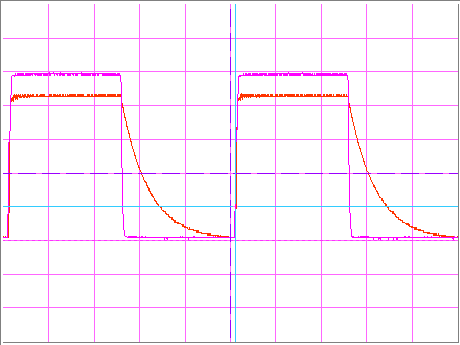
\includegraphics[width = 9cm]{../Obrazki_i_tekst/obrobione/32sciety.png}
    \caption{\( E_F = U_{max}, \ E_R = 0V \) dla częstotliwości 100 kHz }
  \end{center}
\end{figure}

Na tym przebiegu widać, że w podanej częstotliwości dioda już nie pracuje jak dobry włącznik.
\newline
\newline
Następnie przystąpiliśmy do badania kluczy tranzystorowych, za pomocą układu drugiego. 
Otrzymane przebiegi przedstawiamy pod spodem: 
\begin{figure} [H]
  \begin{center}
    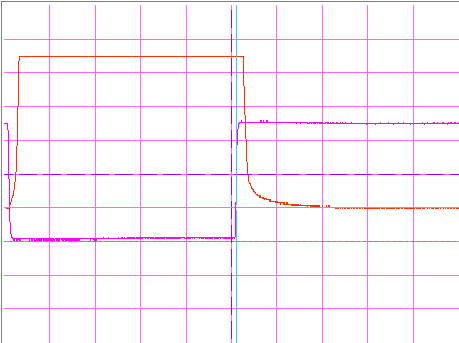
\includegraphics[width = 9cm]{../Obrazki_i_tekst/obrobione/II1ciety.png}
    \caption{Układ bez elementów dodatkowych }
  \end{center}
\end{figure}
\(t_d = 0,2 \mu s,\ t_r = 3 \mu s,\ t_{s} \approx 0 \mu s,\ t_{f} = 0,3 \mu s \).
Ponadto dla każdego przebiegu widzimy też napięcie nasycenia $ U_{CEsat} = 1V $. 

\begin{figure} [H]
  \begin{center}
    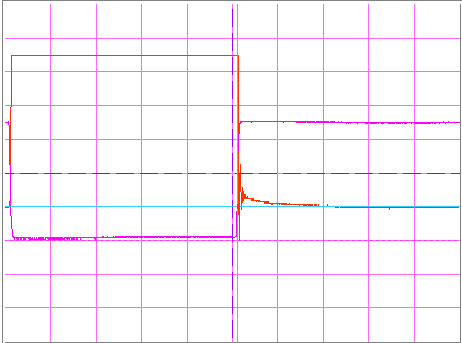
\includegraphics[width = 9cm]{../Obrazki_i_tekst/obrobione/II1zkondecprzyspciety.png}
    \caption{Układ z kondensatorem przyspieszającym $C$}
  \end{center}
\end{figure}
\(t_d = 0 \mu s,\ t_r = 2 \mu s,\ t_{s} = 0 \mu s,\ t_{f} = 0 \mu s \).
\begin{figure} [H]
  \begin{center}
    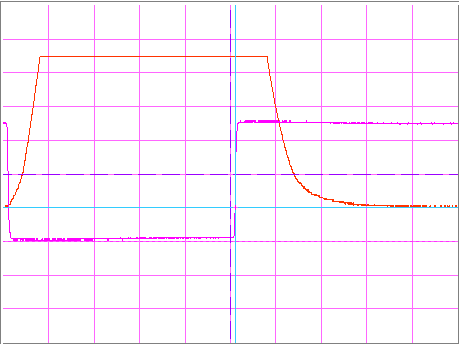
\includegraphics[width = 9cm]{../Obrazki_i_tekst/obrobione/II1zdiodasciety.png}
    \caption{układ z diodą}
  \end{center}
\end{figure}
\(t_d = 0 \mu s,\ t_r = 1,5 \mu s,\ t_{s} = 2 \mu s,\ t_{f} = 4 \mu s \).
Tutaj spotkała nas nie lada niespodzianka. Użycie diody w układzie miało na celu poprawienie jego właściwości, ale stało się inaczej, bo właściwości przełączające się pogorszyły, bo czas przełączania się zwiększył. Wnioskujemy zatem, że dioda nie spełniała w układzie swojej funkcji (miała nie doprowadzać tranzystora do nasycenia).

\begin{figure} [H]
  \begin{center}
    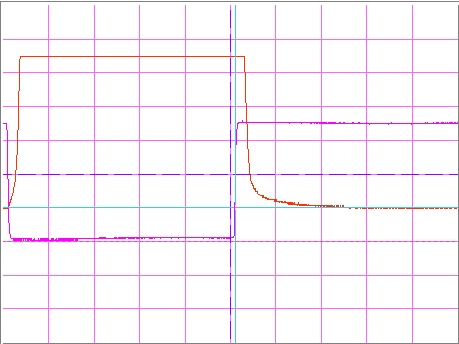
\includegraphics[width = 9cm]{../Obrazki_i_tekst/obrobione/II1zkon2ciety.png}
    \caption{ Układ z kondensatorem obciążającym $C_L$ }
  \end{center}
\end{figure}
\(t_d = 0 \mu s,\ t_r = 0,2 \mu s,\ t_{s} = 0,2 \mu s,\ t_{f} = 2 \mu s \).

\begin{figure} [H]
  \begin{center}
    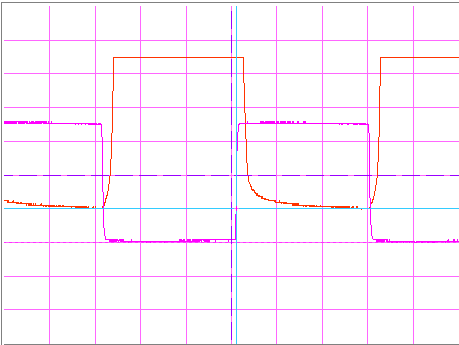
\includegraphics[width = 9cm]{../Obrazki_i_tekst/obrobione/II1zfgranicznaciety.png}
    \caption{ Układ działający przy częstotliwoścu granicznej [ 85 kHz ] z nasyconym tranzystorem }
  \end{center}
\end{figure}
\(t_d = 0 \mu s,\ t_r = 0,3 \mu s,\ t_{s} = 0,2 \mu s,\ t_{f} = 5 \mu s \).


Następnie przystąpiliśmy do badzania układu z przełącznikiem elektromechanicznym. 
Na początku wyznaczaliśmy oporności cewki miernikiem elektronicznym. 
$$ R_l = 406 \Omega, \ R_z = 0,4 \Omega, \ R_r > 20 M\Omega $$ 

Następnie zarejestrowaliśmy następujący przebieg napięcia: 
\begin{figure} [H]
  \begin{center}
    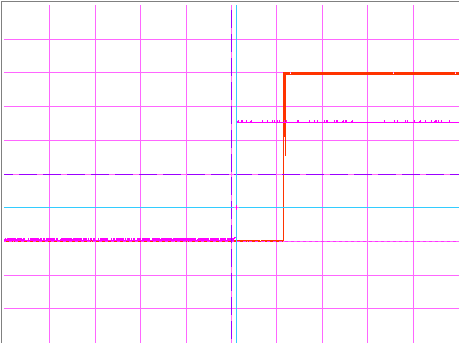
\includegraphics[width = 9cm]{../Obrazki_i_tekst/obrobione/IIIciety.png}
    \caption{ Układ z przełącznikiem elektromechanicznym }
  \end{center}
\end{figure}

Co wyglądało niepokojąco dobrze. Dopiero w powiększeniu widać było specyficzne defekty tego przełącznika: 
\begin{figure} [H]
  \begin{center}
    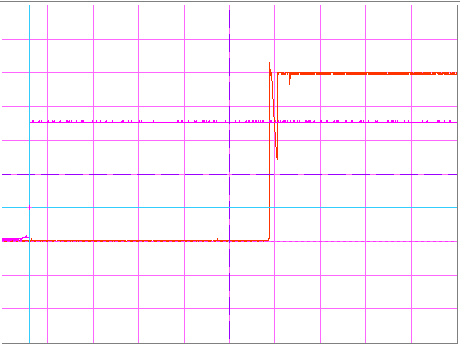
\includegraphics[width = 9cm]{../Obrazki_i_tekst/obrobione/IIIlepsiejszeciety.png}
    \caption{ Układ z przełącznikiem elektromechanicznym }
  \end{center}
\end{figure}

Na powyższym zdjęciu widać wyraźnie zakłócenia przy przełączaniu. A także opóźnienie wyłącznika $t_{off}=5,5 ms$, co jest sporym opóźnieniem w stosunku do innych układow.



%\section{Niepewności}
% pomijamy, bo to nie nie pewnosci a obserwacje są waże w doswiadczeniu!!! ... łomen! : P  
% głównie cewki ... bo co innego + wzory 

\section{Wnioski}

% częstotliwości graniczne 
% uklady dobre w odpowiednich czestotliwosciach 
% od teraz zawsze bedziem cos włączać, bądź wyłączać, bo to kochamy ! 
Nie ma idealnych przełączników. Na rynku możey jedynie wybierać spośród takich, które mają większe będź mniejsze zalety, w zależmości od potrzeb. Tak oto: 
\begin{itemize}
  \item Przełączniki diodowe i tranzystorowe przy dużych częstotliwościach tracą swoje właściwości 
  \item Przełącznik elektromechaniczny ma bardziej strome przejścia z pozycji włączonej do wyłączonej, ale w zamian za to przy mechanicznym przełączaniu występuje spore  opóźnienie, i dość nieprzewidywalne skoki napięcia przy przekoku przełącznika. 
  \item Przełącznik elektromechaniczny pracuje tylko na niskich częstotliwościach 
  \item Przełączniki diodowe i tranzystorowe zachowują się inaczej, gdy do układu dodamy inne elementu co zdecydowanie polepsza właściwości przełącznika. 
\end{itemize}

\end{document}
